
Mary and Alice are buying items for Sunday lunch. Mary buys either chicken $(C)$ or beef $(B)$ for the main course and Alice buys either juice $(J)$ 
or wine $(W)$. Both people prefer wine with beef and juice with chicken. The opposite alternatives are equally displeasing.
However, Mary prefers beef over chicken, while Alice prefers chicken over beef.

We assume that Mary buys first and then tells Alice what she bought,
so when Alice makes her decision, she knows if the main course is beef or chicken.

\begin{enumerate}
    \item[(a)] Express the above preferences as payoffs by using numbers\\
    (e.g. $u_M(B, W) = 2$, $u_A(B, W) = \ldots$  etc.) \hfill{\bf [2 marks]}\smallskip

    As Mary prefers $B$ over $C$, and Alice prefers $C$ over $B$, $u_M(B, W) > u_A(B, W)$ and $u_M(C, J) < u_A(C, J)$.
    As both prefer $B$ with $W$ and $C$ with $J$, $u_i(B, W) > 0, u_i(C, J) > 0 : i \in \{M, A\}$
    As both are equally displeased by $B$ with $J$ and $C$ with $W$, $u_i(B, J) = u_i(C, W), u_i(B, J) < u_i(B, W), u_i(C, W) < u_i(B, J) : i \in \{M, A\}$

    The following assignment satisfies these constraints:
    \begin{equation}
        \begin{split}
            u_M(B, W) = 2, u_A(B, W) = 1, \\
            u_M(B, J) = 0, u_A(B, J) = 0, \\
            u_M(C, W) = 0, u_A(C, W) = 0, \\
            u_M(C, J) = 1, u_A(C, J) = 2
        \end{split}
    \end{equation}

    \item[(b)] Write down a bimatrix game with Mary as the row player and Alice as the column player, using your chosen payoffs. \hfill{\bf [4 marks]}\smallskip

    \begin{table}[ht!]
        \centering
        \begin{tabular}{lc|cl|cl|}
        \cline{3-6}
         &  & \multicolumn{4}{c|}{Alice}                      \\ \cline{3-6} 
         &  & \multicolumn{2}{c|}{J} & \multicolumn{2}{c|}{W} \\ \hline
        \multicolumn{1}{|c|}{\multirow{2}{*}{Mary}} & C                      & 1                     & \multicolumn{1}{c|}{2} & 0                     & \multicolumn{1}{c|}{0} \\ \cline{2-6} 
        \multicolumn{1}{|c|}{}                      & \multicolumn{1}{l|}{B} & \multicolumn{1}{l}{0} & 0                      & \multicolumn{1}{l}{2} & 1                      \\ \hline
        \end{tabular}
        \caption{Bimatrix game representation of the scenario in Exercise 3}
        \label{tab:ex3b}
    \end{table}

    \item[(c)] Write down a game tree representing this game as an extended game.  \hfill{\bf [4 marks]}\smallskip

    As Mary buys first, she is at the root of the tree, the two outward edges represent the choice between $B$ and $C$.
    Whether $B$ or $C$ is chosen, Alice is the next node, these each have two edges representing the choice between $W$ and $J$.
    Finally, the leaves represent the payoffs for each player from the corresponding actions taken from the root to the leaf.

    \hfil
    \begin{tikzpicture}[level distance=36pt,sibling distance=12pt]
    \Tree [.Mary
        \edge node[auto=right]{$B$};
        [.Alice
        \edge node[auto=right]{$W$}; $2,1$
        \edge node[auto=left]{$J$}; $0,0$ ]
        \edge node[auto=left]{$C$};
        [.Alice
        \edge node[auto=right]{$W$}; $0,0$
        \edge node[auto=left]{$J$}; $1,2$ ]
    ]
    \end{tikzpicture}
    \hfil

    \item[(d)] Find a solution for the extended game using backward induction.\\Describe your steps.  \hfill{\bf [5 marks]}\smallskip

    For this solution, an edge with a solid line represents the action that is chosen. 

    Firstly consider the left subgraph (taking action $B$), Alice may either choose $W$ with reward $1$ or $J$ with reward $0$.
    As $1 > 0$, Alice chooses $W$ and her node takes the payoff value $2,1$.

    \hfil
    \begin{tikzpicture}[level distance=36pt,sibling distance=12pt]
    \Tree [.\text{Alice ($2,1$)}
        \edge node[auto=right]{$W$}; $2,1$
        \edge[dashed] node[auto=left]{$J$}; $0,0$
    ]
    \end{tikzpicture}
    \hfil

    Next, return to the root and consider its right subgraph (taking action $C$), Alice may either choose $W$ with reward $0$ or $J$ with reward $2$.
    As $0 < 2$, Alice chooses $W$ and her node takes the payoff value $1,2$.

    \hfil
    \begin{tikzpicture}[level distance=36pt,sibling distance=12pt]
    \Tree [.\text{Alice ($1,2$)}
        \edge[dashed] node[auto=right]{$W$}; $0,0$
        \edge node[auto=left]{$J$}; $1,2$
    ]
    \end{tikzpicture}
    \hfil

    Finally, consider the root. Mary may either choose $B$ with reward $2$ or $C$ with reward $1$.
    As $2 > 1$, Alice chooses $B$.

    \hfil
    \begin{tikzpicture}[level distance=36pt,sibling distance=12pt]
    \Tree [.\text{Mary ($2,1$)}
        \edge node[auto=right]{$B$}; $2,1$
        \edge[dashed] node[auto=left]{$C$}; $1,2$
    ]
    \end{tikzpicture}
    \hfil

    The full annotated graph is as follows.

    \hfil
    \begin{tikzpicture}[level distance=36pt,sibling distance=12pt]
    \Tree [.\text{Mary ($2,1$)}
        \edge node[auto=right]{$B$};
        [.\text{Alice ($2,1$)}
        \edge node[auto=right]{$W$}; $2,1$
        \edge[dashed] node[auto=left]{$J$}; $0,0$ ]
        \edge[dashed] node[auto=left]{$C$};
        [.\text{Alice ($1,2$)}
        \edge[dashed] node[auto=right]{$W$}; $0,0$
        \edge node[auto=left]{$J$}; $1,2$ ]
    ]
    \end{tikzpicture}
    \hfil

    Hence, by backwards induction, Mary gets a higher payoff than Alice and they have Beef with Wine for Sunday lunch.

\end{enumerate}
\vspace*{0.8cm}
